\section{Implementation}

\subsection{Anti-windup}

Real electromechanical systems has saturations on their physical variables. In particular,
the output of any actuator is limited from above and below. (Clipping).
If you stay between the limits, the system will behave as a linear system.

\textbf{Back-calculation}

An anti-windup scheme that recomputes the integral term when the system
input is saturated. The value of the integrator output is not changed instantaneously, but it is changed
based on the tracking time constant.

\begin{center}
	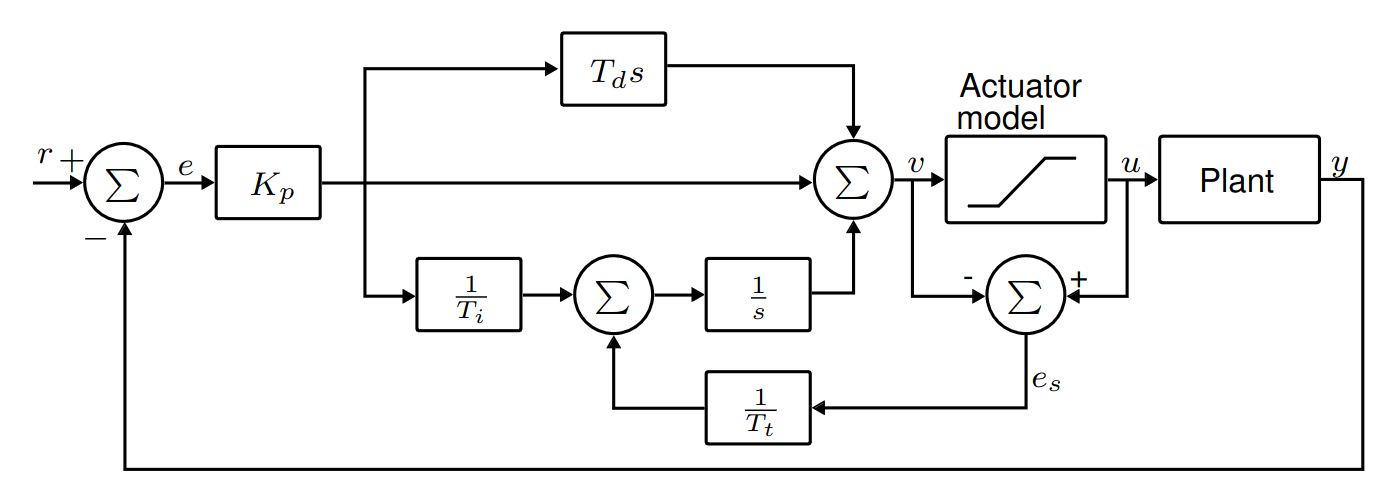
\includegraphics[width = 0.8\textwidth]{Images/backCalc.png}
\end{center}

The input to the integrator is given by
$$ \frac{1}{T_t}e_s  + \frac{K_p}{T_i}e $$

Where $e_s$ is zero when the system is not saturated. In steady state, the output of the integrator is constant:
hence, its input must be zero, i.e.

$$ e_s = -\frac{K_p T_t}{T_i}e $$


\textbf{Conditional integration}

Also known as clamping is a bit simpler, and just stops integreating when the system is in saturation.
\begin{center}
	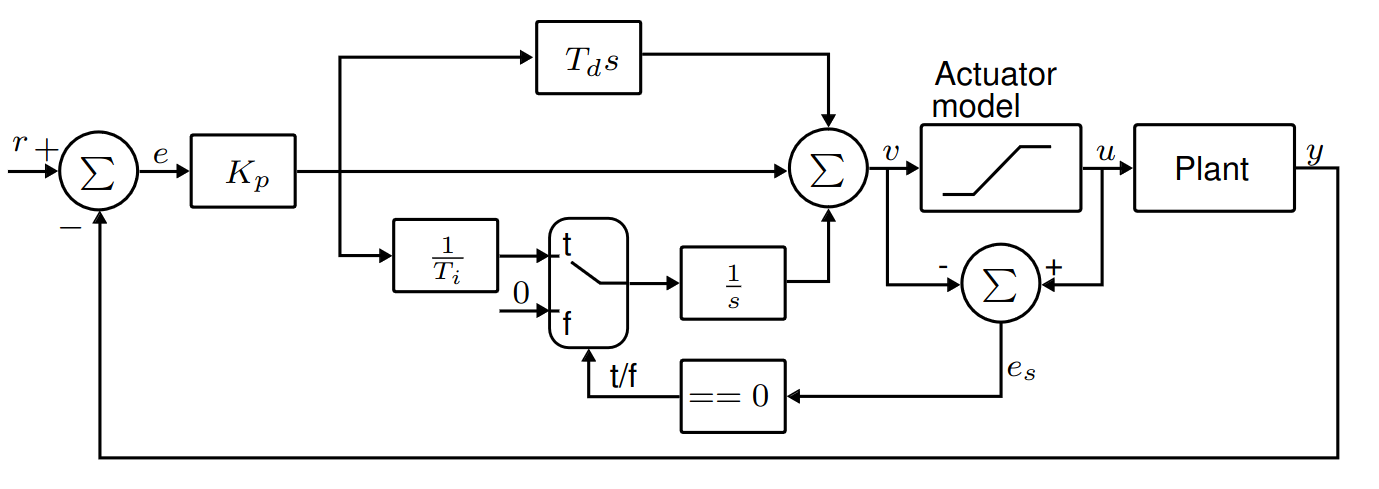
\includegraphics[width=0.7\textwidth]{Images/conditional-integration.png}
\end{center}


\textbf{Setpoint weighting}

To avoid large control signals when changing the reference rapidly, setpoint weiths can be introduced.
These modify the PID controller to be:

$$ u(t) = K_p(\beta r(t) -y(t)) + K_i \int_0^t (r(\tau)-y(\tau))d\tau + K_d (\gamma \frac{dr}{dt} - \frac{dy}{dt})$$

where $\gamma \text{and} \beta$ are setpoint weights. Typically $\gamma = 0$ and $\beta$ takes values between
0 and 1.

\textbf{Filtering}

To avoid large control signal noise on the measured output $y$, one adds a filter
on the derivative term. Often a first order filter is sufficient, but this is application dependent.

$$ u_d = k_d s \frac{1}{1+sT_f}$$

Sometimes it is favorable to filter the control signal directly, thus the controller gets the form
$$ C(s) = K_p (1+\frac{1}{sT_i}+sT_d) \frac{1}{1+sT_f+(sT_f)^2/2}$$

\subsection{Digitalization}
Most control systems are sample data systems, i.e., they consist of both discrete and continous signals.
The sampling frequency used for the discrete controlelr should be above 20 times the closed-loop bandwidth.


\subsubsection{Emulation}
Design continous controller $K(s)$ and approximate it with $K(z)$ obtained via e.g. Tustin's method.
Tustin's method also called the trapezoidal rule means to replace the variable $s$ with $$\frac{2}{T} \frac{z-1}{z+1}$$


The control output of the discrete PID controller can be written using 3 terms.

$$u_p(kT+T) = k_p e(kT+T)$$
$$u_I(kT+T) = u_I(KT)+K_i \frac{T}{2} (e(kT+T)+e(kT))$$
$$u_D(kT+T) = k_D \frac{2}{T} (e(kT+T)-e(kT))-u_D(kT)$$

$$u(kT+T) = u_p(kT+T)+u_I(kT+T)+u_D(kT+T)$$

To analyze the system, the I-term and D-term are z-transformed:
$$z u_I(z) = u_I(z) + k_i \frac{T}{2} (ze(z)+e(z))$$
$$z u_D(z) = k_D \frac{2}{T} (ze(z)-e(z))-u_D(z)$$

This gives the following expression for the controller
$$u(z) = (k_P+k_I \frac{T}{2} \frac{z+1}{z-1}+k_D \frac{2}{T} \frac{z-1}{z+1})e(z)$$


\textbf{Compensation for sampling effects}

\newpage
\textbf{Design procedure}

A discrete controller can be designed by emulation for the system $G(s)$ according to the next procedure:

\begin{enumerate}
	\item{Design continuous compensation for the system $G_d(s)G(s)$, where $G_d(s)$ approximates a delay of $T/2$}
	\item{Derive the discrete controller by applying Tustin's rule or the matched pole-zero method}
	\item{Analyze the design by simulation or experimentally}
\end{enumerate}



\subsubsection{Numerical Integration Methods}
There is three methods to convert a continous controller to a discrete controller:
\begin{center}
	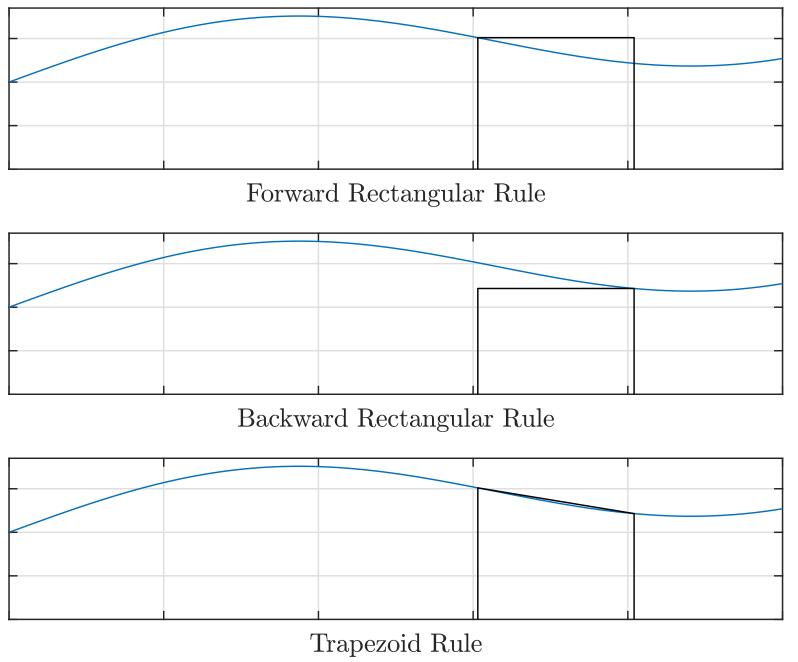
\includegraphics[width=0.5\textwidth]{Images/Numerical-Integration.png}
\end{center}
Get an approximation of the discrete transfer function by replacing $s$ with:
$$\begin{array}{cc}
  \textbf{Method:}& \textbf{Approximation:} \\
  \text{Forward rule:}& s\gets\frac{z-1}{T} \\
  \text{Backward rule:}& s\gets\frac{z-1}{Tz} \\
  \text{Trapezoidal rule:}& s\gets\frac{2}{T} \frac{z-1}{z+1}
\end{array}$$

Get an approximation of the discrete transfer function by replacing $z$ with:
$$\begin{array}{cc}
  \textbf{Method:}& \textbf{Approximation:} \\
  \text{Forward rectangular rule:}& z\gets 1+Ts \\
  \text{Backward rectangular rule:}& z\gets \frac{1}{1-Ts} \\
  \text{Bilinear rule:}& z\gets \frac{1+Ts/2}{1-Ts/2}
\end{array}$$

The left half-plane is mapped to different regions in the $z$-plane for the different methods.
\begin{center}
	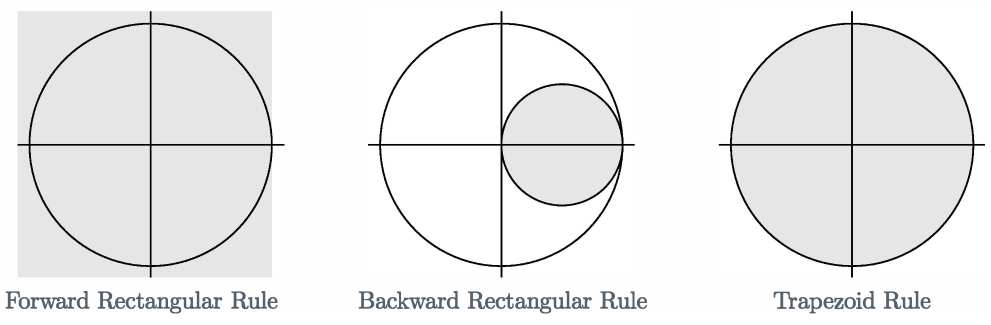
\includegraphics[width=0.8\textwidth]{Images/digitization-mapping.png}
\end{center}
This means that the discretization of a stable system using the forward rule can result in an unstable system.




\subsubsection{Discrete Design}
Design the discrete controller directly, without computing $K(s)$ first.
Therefore it relies on a discretized plant model. The discrete transfer function of a system $G(s)$ and preceding
zero-order hold is
$$G(z) = (1-z^{-1}) Z  \left\{\frac{G(s)}{s}\right\}$$
where $Z$ denotes the Z-transform.

The system can subsequently be analyzed based on the clode-loop transfer function:
$$T_{cl}(z)=\frac{G(z)K(z)}{1+G(z)K(z)}$$
Since the structure of the continuous and discrete closed-loop transfer functions are the same, the stability of the system can be studied via the characteristic equation:
$$1+G(z)K(z)=0$$
Consequently, the controller K(z) can be designed via root locus or any of the other methods.

\textbf{Design procedure}
\begin{enumerate}
  \item Transform the continuous-time plant into discrete time as follows:
    $$G_d(z) = (1-z^{-1}) Z  \left\{\frac{G(s)}{s}\right\}$$
  \item Design the feedback controller $K(z)$ using the same approaches as for a continuous-time.
  \item Verify the design on the sampled data system.
\end{enumerate}

\subsection{Examples}

\textbf{Emulation example of PID controller}

$$K(s) = 1.4 \frac{s+6}{s}$$
Use Tustin's method to emulate the controller in discrete time.
$$K(z) = K(\frac{2}{T} \frac{z-1}{z+1}) = 1.4 \frac{\frac{2}{T} \frac{z-1}{z+1}+6}{\frac{2}{T} \frac{z-1}{z+1}}
	= 1.4 \frac{(1+3T)z-(3T-1)}{z-1}$$

In practice you implement the difference equation - not a discrete transfer function.
